% !TEX root = omar-thesis-proposal.tex
\newcommand{\lamA}{\lambda_{\text{A}}}

\newcommand{\tvarCtx}{\Delta}
\newcommand{\fCtx}{\Sigma}
\newcommand{\itvarCtx}{\Omega}
\newcommand{\iCtx}{\Theta}
\newcommand{\eCtx}{\Gamma}
\newcommand{\etvarCtx}{\Omega}
\newcommand{\fSpec}[3]{\tof{\fvar{#1}}{\kFam{#2}{#3}}}
\newcommand{\fSpecStd}{\fSpec{fam}{\kappaidx}{\Theta}}

\newcommand{\errCtx}{\mathcal{E}}
\newcommand{\famEvalCtx}{\Xi}

% Generic stuff
\newcommand{\pipe}{~\text{\large $\vert$}~}
\newcommand{\splat}[3]{#1_{#2},\ldots,#1_{#3}}
\newcommand{\splatC}[3]{#1_{#2}~~~~\cdots~~~~#1_{#3}}
\newcommand{\splatTwo}[4]{#1_{#3}#2_{#3},~\ldots~, #1_{#4}#2_{#4}}
\newcommand{\substn}[2]{[#1]#2}

% \psi
\newcommand{\psiu}[1]{{\psi_{#1}}}
\newcommand{\psit}[1]{{\psi_{\text{#1}}}}
\newcommand{\psitype}{\psit{type}}
\newcommand{\psiproof}{\psit{proof}}
\newcommand{\psiidx}{\psit{idx}}
\newcommand{\psiidxn}[1]{\psit{idx,#1}}
\newcommand{\psirep}{\psit{rep}}
\newcommand{\psirepn}[1]{\psit{rep,#1}}
\newcommand{\psiden}{\psit{den}}
\newcommand{\psiIT}{\psit{IT}}
\newcommand{\psiarrow}{\psit{arrow}}
\newcommand{\psiprod}{\psit{prod}}
\newcommand{\psiint}{\psit{int}}
\newcommand{\psibool}{\psit{bool}}
\newcommand{\psiprog}{\psit{prog}}
\newcommand{\psiiterm}{\psit{iterm}}

% \delta
\newcommand{\delt}[1]{\delta_{\text{#1}}}
\newcommand{\delrep}{\delt{rep}}

% \kappa
\newcommand{\kappat}[1]{\kappa_{\text{#1}}}
\newcommand{\kappaidx}{\kappat{idx}}

% Expressions
\newcommand{\expr}[1]{{\color{red} #1}}
\newcommand{\elam}[3]{{\lam{#1}{#2}{#3}}}
\newcommand{\evar}[1]{{\textrm{#1}}}
\newcommand{\eapp}[2]{{#1~#2}}
\newcommand{\eop}[4]{{#1.\tvar{#2}\langle#3\rangle(#4)}}

% Types
\newcommand{\tdef}[3]{{\sf def}~\tvar{#1}=#2~{\sf in}~#3}
\newcommand{\tlam}[2]{\lambda#1.#2}
\newcommand{\tvar}[1]{{\textbf{#1}}}
\newcommand{\tapp}[2]{#1(#2)}
\newcommand{\tifeq}[4]{{\sf if}~#1\equiv#2~{\sf then}~#3~{\sf else}~#4}

\newcommand{\tunit}{()}
\newcommand{\tpair}[2]{(#1, #2)}
\newcommand{\tfst}[1]{{\sf fst}~#1}
\newcommand{\tsnd}[1]{{\sf snd}~#1}

\newcommand{\fvar}[1]{\textsc{#1}}
\newcommand{\tfam}[6]{{\sf family}~\fvar{#1}[#2]~::~#3~\{#4 : #5\}~{\sf in}~#6}
\newcommand{\tfamStd}{\tfam{fam}{\kappaidx}{\psirep}{\theta}{\Theta}{\psi}}
\newcommand{\tfamcase}[4]{{\sf famcase}~#1~{\sf of}~#2~{\sf then}~#3~{\sf else}~#4}
\newcommand{\tfamSpec}[5]{{\sf family}~[#2]~::~#3~\{#4 : #5\}}
\newcommand{\tfamSpecStd}{\tfamSpec{fam}{\kappaidx}{\psirep}{\theta}{\Theta}}

\newcommand{\ttype}[2]{{\sf type}[#1]\in#2}
\newcommand{\ttypestd}{\ttype{\psiidx}{\phi}}
\newcommand{\tidx}[1]{{\sf idxof}~#1}
\newcommand{\trepof}[1]{{\sf repof}~#1}

\newcommand{\tden}[2]{\llbracket #1 \sim #2 \rrbracket}
\newcommand{\ttypeof}[1]{{\sf typeof}~#1}
\newcommand{\tvalof}[1]{{\sf valof}~#1}
\newcommand{\terr}{{\sf err}}
\newcommand{\tdencase}[4]{{\sf dencase}~#1~{\sf of}~#2~{\sf then}~#3~{\sf else}~#4}

\newcommand{\titerm}[1]{{\sf iterm}(#1)}
\newcommand{\titype}[1]{{\sf itype}(#1)}

\newcommand{\tconst}[1]{{\sf const}(#1)}
\newcommand{\tOp}[1]{{\sf op}(#1)}

\newcommand{\tprog}[1]{{\sf program}(#1)}

\newcommand{\topsempty}{\cdot}
\newcommand{\tops}[2]{\tvar{#1}=#2}
\newcommand{\topp}[2]{#1; #2}
\newcommand{\Tops}[2]{\tvar{#1} : #2}
\newcommand{\Topp}[2]{#1; #2}
\newcommand{\Toppstd}{\Topp{\Theta'}{\Tops{id}{
			\karrow{
				\kType{\kFamStd}
			}{
				\karrow{
					\splat{\kappa}{1}{m}
				}{
					\kOp{n}
				}
			}
		}}
}

% IL terms
\newcommand{\ivar}[1]{\textrm{#1}}
\newcommand{\ilam}[3]{\lambda #1::#2.#3}
\newcommand{\ifix}[3]{{\sf fix~}#1::#2.#3}
\newcommand{\iapp}[2]{#1~#2}
\newcommand{\ipair}[2]{(#1, #2)}
\newcommand{\ifst}[1]{{\sf fst}~#1}
\newcommand{\isnd}[1]{{\sf snd}~#1}
\newcommand{\iintlit}{n}
\newcommand{\iop}[2]{#1 + #2}
\newcommand{\iIfEq}[4]{{\sf if}~#1\equiv#2~{\sf then}~#3~{\sf else}~#4}
\newcommand{\mvalof}[1]{{\sf valof}(#1)}
\newcommand{\iup}[1]{\uparrow(#1)}

% Internal Types
\newcommand{\darrow}[2]{#1\rightarrow#2}
\newcommand{\dint}{\texttt{int}}
\newcommand{\dpair}[2]{#1\times#2}
\newcommand{\dup}[1]{\uparrow(#1)}
\newcommand{\drepof}[1]{{\sf repof}(#1)}

% Kinds
\newcommand{\kvar}[1]{\textrm{#1}}
\newcommand{\karrow}[2]{#1\rightarrow{#2}}
\newcommand{\kforall}[2]{\forall \kvar{#1}.#2}
\newcommand{\kunit}{\texttt{Unit}}
\newcommand{\kstr}{\texttt{Str}}
\newcommand{\kpair}[2]{#1 \times #2}
\newcommand{\klabel}[1]{\textsc{#1}}
\newcommand{\klabelOf}[2]{\klabel{#1}~{\tt of}~#2}
\newcommand{\kTypeBlur}{\texttt{Type}}
\newcommand{\kType}[1]{\texttt{Type}\in #1}
\newcommand{\kOp}[1]{\texttt{Op}_{#1}}
\newcommand{\kDen}{\texttt{Den}}
\newcommand{\kDenk}[1]{\texttt{Den}[#1]}
\newcommand{\kIdxcase}[1]{{\tt Idxcase}~#1}
\newcommand{\kIType}{\texttt{IType}}
\newcommand{\kITerm}{\texttt{ITerm}}
\newcommand{\kEqProof}[3]{#1 \equiv_{#2} #3}
\newcommand{\kProg}{\texttt{Program}}
\newcommand{\kcasev}{\Omega^n}
\newcommand{\kFam}[2]{{\tt family}[#1]\{#2\}}
\newcommand{\kFamStd}{\kFam{\kappaidx}{\Theta}}
\newcommand{\kFamVar}[1]{\overline{\fvar{#1}}}

% Judgements
\newcommand{\tof}[2]{#1 : #2}
\newcommand{\mtof}[2]{#1 :: #2}
\newcommand{\tentails}[2]{#1 \vdash #2}
\newcommand{\tentailst}[3]{\tentails{#1}{\tof{#2}{#3}}}
\newcommand{\tStdCtx}{\fCtx~\tvarCtx}
\newcommand{\tCtxXF}[1]{\fCtx, #1~\tvarCtx}
\newcommand{\tCtxXT}[1]{\fCtx~\tvarCtx, #1}
%\newcommand{\tCtxXL}[1]{\fCtx~\tvarCtx~\lvarCtx, #1}
\newcommand{\tentailsX}[1]{\tentails{\tStdCtx}{#1}}
\newcommand{\tentailsXt}[2]{\tentailsX{\tof{#1}{#2}}}
\newcommand{\kentails}[2]{#1 \vdash #2}
\newcommand{\kentailsX}[1]{\kentails{\fCtx}{#1}}
\newcommand{\iMkCtx}[3]{#1~#2~#3}
\newcommand{\iStdCtx}{\iMkCtx{\fCtx}{\tvarCtx}{\itvarCtx}}
\newcommand{\ientails}[2]{#1 \vdash #2}
\newcommand{\ientailsX}[1]{\entails{\iStdCtx}{#1}}
\newcommand{\casemap}[2]{#1 : #2}
\newcommand{\mentails}[3]{#1, #2 \vdash #3}
\newcommand{\mentailsX}[1]{\mentails{\tvarCtx}{\itvarCtx}{#1}}
\newcommand{\eentails}[4]{#1~#2~#3 \vdash #4}
\newcommand{\eentailsX}[1]{\eentails{\fCtx}{\tvarCtx}{\etvarCtx}{#1}}
\newcommand{\mtentails}[2]{#1 \vdash #2}
\newcommand{\mtentailsX}[1]{\mtentails{\iCtx}{#1}}
\newcommand{\mtentailsXt}[2]{\mtentails{\iCtx}{\mtof{#1}{#2}}}
\newcommand{\kSimple}[1]{#1~{\sf simple}}
\newcommand{\Tentails}[3]{#1 \vdash_{#2} #3}
\newcommand{\TentailsX}[1]{\Tentails{\fCtx}{\fvar{fam}}{#1}}

% Big-Step Semantics
\newcommand{\tevals}[4]{\entails{#1}{#2 \curlyveedownarrow_{#4} #3}}
\newcommand{\tevalsX}[3]{\tevals{\famEvalCtx}{#1}{#2}{#3}}
\newcommand{\tevalX}[2]{\tevalsX{#1}{#2}{\errCtx}}
\newcommand{\tevalms}[3]{#1 \curlyveedownarrow_{#3} #2}
\newcommand{\tevalm}[2]{\tevalms{#1}{#2}{\errCtx}}
\newcommand{\tevales}[3]{#1 \curlyveedownarrow_{#3} #2}
\newcommand{\tevale}[2]{\tevales{#1}{#2}{\errCtx}}
\newcommand{\noprob}{\text{ok}}
\newcommand{\prob}{!}

% Verification and Translation
\newcommand{\translates}[4]{\entails{#1}{#2 \longrightarrow \tden{#3}{#4}}}

% Compilation Semantics
\newcommand{\compiless}[3]{#1 \Longrightarrow \tden{#2}{#3}}
\newcommand{\compiles}[3]{#1 \Longrightarrow \tden{#2}{#3}}
%\newcommand{\translates}[6]{\entails{#1}{\translatesTo{#2}{#3}{#4}{#5}{#6}}}
\newcommand{\translatesTo}[5]{#1 \longrightarrow \tden{#2}{\ttype{#3}{#4}{#5}{6}{7}}}
\newcommand{\translatesX}[5]{\translates{\eCtx}{#1}{#2}{#3}{#4}{#5}}

% !TEX root = omar-thesis-proposal.tex
\newcommand{\lam}[3]{\lambda #1{:}#2.#3}
\newcommand{\ap}[2]{#1~#2}
\newcommand{\z}{\textsf{z}}
\newcommand{\s}[1]{\textsf{s}(#1)}
\newcommand{\natrec}[5]{\textsf{natrec}(#1; #2; #3,#4.#5)}
\newcommand{\pair}[2]{(#1, #2)}
\newcommand{\fst}[1]{\textsf{fst}(#1)}
\newcommand{\snd}[1]{\textsf{snd}(#1)}

\newcommand{\tArrow}[2]{#1 \rightarrow #2}
\newcommand{\nat}{\texttt{nat}}
\renewcommand{\prod}[2]{#1 \times #2}

%\newcommand{\eCtx}{\Gamma}
\newcommand{\eCtxX}[3]{#1, #2 : #3}
\newcommand{\jet}[3]{#1 \vdash #2 : #3}
\newcommand{\jetX}[2]{\jet{\eCtx}{#1}{#2}}

\lstset{language=ML,
basicstyle=\ttfamily\footnotesize,
morekeywords={newcase,extends},
}

\section{Active Typechecking and Translation}\label{att}

In this section, we will restrict our focus to actively-typed mechanisms for implementing extensions to the static and dynamic semantics of programming languages. Programming languages are typically designed around a monolithic collection of primitive type families and operators. Consider, as a simple example, G\"odel's T \cite{pfpl}, a typed lambda calculus with recursion on primitive natural numbers (Figure \ref{T}). Although a researcher may casually speak of ``extending G\"odel's T with primitive product types'' (Figure \ref{prods}), modularly adding this new primitive type family and its corresponding operators to this language from within is impossible. That is, G\"odel's T is not \emph{internally extensible}.

\begin{figure}
\small
\begin{mathpar}
\inferrule[var]{ }{
	\jet{\eCtxX{\eCtx}{x}{\tau}}{x}{\tau}
}

\inferrule[Arrow-I]{
	\jet{\eCtxX{\eCtx}{x}{\tau}}{e}{\tau'}	
}{
	\jetX{\lam{x}{\tau}{e}}{\tArrow{\tau}{\tau'}}
}

\inferrule[Arrow-E]{
	\jetX{e_1}{\tArrow{\tau}{\tau'}}\\
	\jetX{e_2}{\tau}
}{
	\jetX{\ap{e_1}{e_2}}{\tau'}
}

\inferrule[Nat-I1]{ }{
	\jetX{\z}{\nat}
}

\inferrule[Nat-I2]{
	\jetX{e}{\nat}
}{
	\jetX{\s{e}}{\nat}
}

\inferrule[Nat-E]{
	\jetX{e_1}{\nat}\\
	\jetX{e_2}{\tau}\\
	\jet{\eCtxX{\eCtxX{\eCtx}{x}{\nat}}{y}{\tau}}{e_3}{\tau}
}{
	\jetX{\natrec{e_1}{e_2}{x}{y}{e_3}}{\tau}
}
\end{mathpar}
\caption{Static semantics of G\"odel's T}\label{T}
\end{figure}
\begin{figure}
\small
\begin{mathpar}
\inferrule[Prod-I]{
	\jetX{e_1}{\tau_1}\\
	\jetX{e_2}{\tau_2}
}{
	\jetX{\pair{e_1}{e_2}}{\prod{\tau_1}{\tau_2}}
}

\inferrule[Prod-E1]{
	\jetX{e}{\prod{\tau_1}{\tau_2}}
}{
	\jetX{\fst{e}}{\tau_1}
}

\inferrule[Prod-E2]{
	\jetX{e}{\prod{\tau_1}{\tau_2}}
}{
	\jetX{\snd{e}}{\tau_2}
}
\end{mathpar}
\caption{Static semantics of products}\label{prods}
\end{figure}
The only recourse researchers have in such situations is to attempt to define new constructs in terms of existing constructs. Such encodings, collections of which are often called \emph{embedded domain-specific languages (DSLs)} \cite{fowler2010domain}, must creatively combine the constructs available in the host ``general-purpose'' language. Unfortunately, such encodings can be difficult to conceive of and impractical or impossible in some cases. For our example of adding products to G\"odel's T, a full encoding is impossible. Limited forms of Church encodings are possible, where products are represented by lambda terms, but they require a reasonable level of creativity\footnote{Anecdotally, Church encodings in System F  were among the more challenging topics for students in our undergraduate programming languages course, 15-312. Note that System F, because it includes type abstraction (that is, parametric polymorphism), supports stronger encodings of types like products than System T does. But products are still only weakly definable in System F and the same fundamental problems discussed above occur.} and in doing so, the type system cannot enforce a distinction between product types and the function types they are encoded using. It is also more difficult to reason about products represented in this way (for example, they will not have unique canonical forms in the same situations)\todo{cite the stuff Bob mentioned on universality}. This strategy will also likely incur a performance penalty because it uses closures rather than a more direct and better optimized internal representation. 

This is not only a problem for minimal languages like G\"odel's T. Several embedded DSLs for Haskell and Scala have also needed to make significant compromises at times. For example... \todo{Scala/Delite examples? Haskell GPU thing?}

%creating a new language. If this is not practical, the best one can attempt to do is encode the new types in terms of existing types (by a Church encoding, for example). This is generally unsatisfactory -- 

%Languages implemented using these common patterns are central planning by a language designer or design committee. 

%Researchers or domain experts who cannot work around such limitations must develop new standalone languages. In our simple scenario, we may simply copy our implementation of G\"odel's T or even edit it directly (a pernicious technique for implementing a new language where the prior one is overwritten). In a more complex scenario, we may instead employ a tool like a compiler generator or DSL framework \cite{fowler2010domain} that can generate a standalone implementation from declarative specifications of language constructs. Some of these tools allow you to package and reuse these specifications (with the important caveat that not all combinations of constructs are valid and free of conflicts, an important modularity issue that we will return to several times in this paper).
%
%The increasing sophistication and ease-of-use of these tools have led many to suggest a {\it language-oriented approach} \cite{journals/stp/Ward94} to software development where different components of an application are written in different languages. Unfortunately, this leads to problems at language boundaries: a library's external interface must only use constructs that can reasonably be expressed in \emph{all possible calling languages}. This can restrict domain-specific languages by, for example, precluding constructs that rely on statically-checked invariants stronger than those their underlying representation in a common target language normally supports. At best, constructs like these can be exposed by generating a wrapper where run-time checks have been inserted to guarantee necessary invariants. This compromises both verifiability and performance and requires the development of an interoperability layer for every DSL. Moreover, library clients must work with verbose and unnatural ``glue code'' when interfacing across languages, defeating the primary purpose of high-level programming languages: hiding the low-level details from the end-users of abstractions. We diagram this fundamental \emph{compatibility problem} in Figure \ref{approaches}(a).
%\begin{figure*}
%\begin{center}
%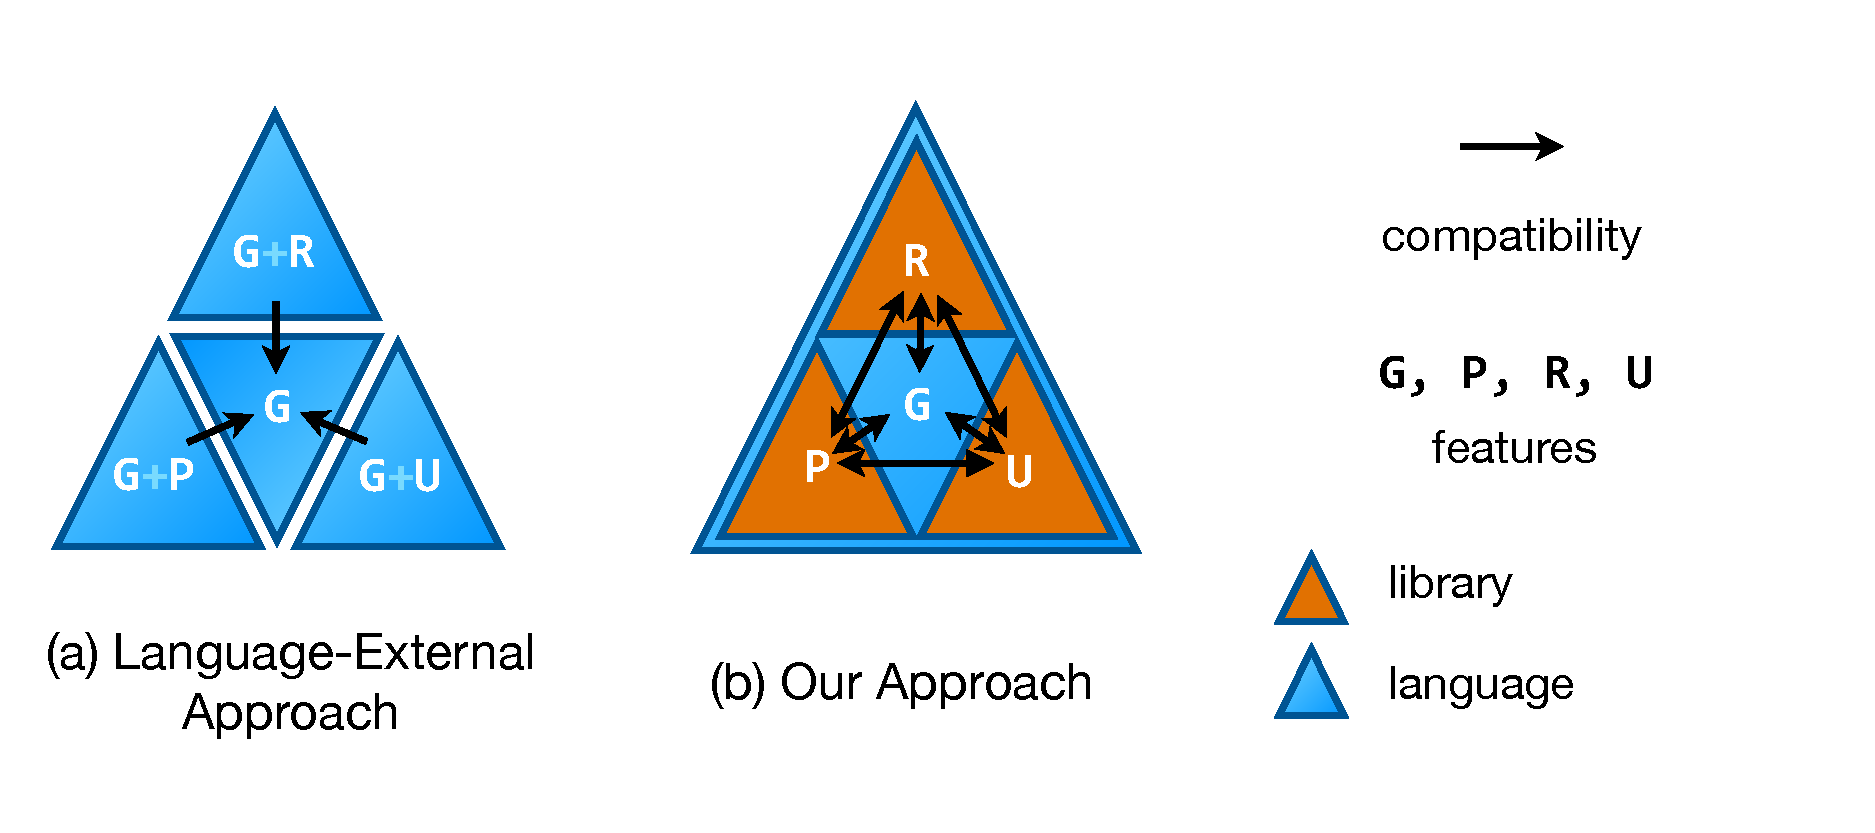
\includegraphics[scale=0.5]{approaches.pdf}
%\end{center}
%\vspace{-20px}
%\caption{\small (a) With a language-oriented approach, novel constructs are packaged into separate languages. Users can only safely and naturally call into languages consisting of common constructs (often only the common target language, such as C or Java bytecode). (b) With a language-internal extensibility approach, there is one system providing a common internal language, where additional primitive constructs that strictly strengthen its static guarantees or perform specialized code generation are specified and distributed within libraries. \label{approaches}}
%\end{figure*}

%As a result, domain-specific languages and new general-purpose abstractions alike have experienced relatively slow adoption in practice.
%
%Porting large codebases to new languages is difficult, and the dominant programming languages innovate slowly, so programming language.
%
%More specifically, such languages are neither \emph{internally extensible} because the language itself exposes only natural numbers and functions to its users, nor are they \emph{externally extensible} because no new behaviors can be added to the language's  implementation in a separate module from the one containing the initial implementation.

%This is the essence of a monolithic language implementation: it is impossible for anyone to modularly extend languages defined in this way. 


An internally-extensible programming language could address these problems by providing a language mechanism for extending, directly, its static and dynamic semantics, so as to support domain-specific type systems and implementation strategies in libraries. 
%Library developers need only consider which abstractions are most appropriate for their domain, without also considering whether these constructs can be exposed using abstractions appropriate to the domains of client code. Clients can simply import any necessary constructs when using a library that relies on them, preserving safety and ease-of-use without the use of  wrappers and glue code. We show this competing approach in Figure \ref{approaches}(b).
%Researchers and domain experts thus gain the ability to distribute new ideas for evaluation to a broader development community without requiring the approval of maintainers of mainstream languages, large-scale porting of code or explicit interoperability layers. 
But, as mentioned in Section \ref{motivation}, some significant challenges must be addressed: balancing  expressiveness with concerns about maintaining various safety properties in the presence of arbitrary combinations of user-defined  extensions. The mechanism must also ensure that desirable metatheoretic properties and global safety guarantees of the language cannot be weakened by extensions. Correctness properties of an extension itself should also be modularly verifiable, so that its users can rely on it for verifying and compiling their own code.  And with multiple independently developed extensions used within one program, the mechanism must further guarantee that they cannot interfere with one another. 

\newpage
\subsection{Theory}\label{atlam}
%\begin{figure}
%\begin{mathpar}
%\inferrule{a}{b}
%\end{mathpar}
%\end{figure}
In this section, we will describe a minimal calculus that captures our language-internal extensibility mechanism,  called \emph{active typechecking and translation (AT\&T)}. AT\&T allows developers to declare new primitive type families, associate operators with them, implement their static semantics in a functional style, and realize their dynamic semantics by simultaneously implementing a translation into a typed internal language. Note that this latter mechanism is closely related to how Standard ML was (re-)specified\todo{cite/read a bit about this/ask Bob/flesh this out}, but that we are fundamentally interested in extending language \emph{implementations}, not their  declarative specifications; proving the adequacy of such implementations against mechanized specifications, or extracting them directly from such specifications, will be investigated in future work.

The AT\&T mechanism utilizes type-level computation of higher kind and integrates typed compilation techniques into the language to allow us to give strong metatheoretic guarantees,  and uses a mechanism notionally related to abstract types (such as those found in the ML module system) to guarantee that extensions cannot interfere with one another,  while remaining straightforward and expressive. In this section, we will develop a core calculus, called \atlam, which uses a minimal, uniform grammar for primitive operators. Then in Section \ref{ace}, we will show how to realize this minimal mechanism within a widely-used language with a more expressive grammar.

%AT\&T is general with respect to many choices about the type-level language, the typed internal language and syntax. Choices along these dimensions can affect both expressiveness and ease-of-use. We will begin in Sec. 2 by introducing a minimal system called $@\lambda$ (the ``actively-typed lambda calculus'') that distills the essence of the mechanism in a simply-typed, simply-kinded setting. This will allow us to fully and concisely formalize the language and compiler and give several key safety theorems. We will then continue in Sec. 3 by discussing variants of this mechanism based on other basic paradigms, considering dependently-typed functional languages and object-oriented languages, discussing trade-offs between expressivity and safety when doing so. We have developed a simple prototype called Ace and have used it to develop a number of full-scale language extensions as libraries. We will briefly discuss this language and these extensions in Sec. 4.

%We note at the outset that AT\&T focuses on extending the static semantics of languages with fixed, though flexible, syntax. Language-internal syntax extension mechanisms have been developed in the past (e.g. SugarJ \cite{sugarj}) but they have also suffered from safety problems because grammar composition is not always safe when done in an  unconstrained manner. Constrained approaches that provide stronger safety guarantees have recently been outlined (e.g. Wyvern \cite{globaldsl13}) but we will leave integration of syntax extensions with semantic extensions as future work.

\subsubsection{From Externally-Extensible Implementations to Internally-Extensible Languages}
To understand the genesis of our internal extensibility mechanism, it is helpful to begin by considering why most implementations of programming languages are not even \emph{externally extensible}. Let us consider again G\"odel's T. 
In a functional implementation, its types and operators will invariably be represented using {closed} datatypes. For example, a simple implementation in Standard ML may be based around these datatypes:
\begin{lstlisting}
datatype Type = Nat | Arrow of Type * Type
datatype Exp = Var of var 
               | Lam of var * Type * Exp
               | Ap of Exp * Exp 
               | Z | S of Exp 
               | Natrec of Exp * Exp * Exp
\end{lstlisting}

The logic governing the typechecking phase as well as the initial compilation phase (we call this phase \emph{translation} to distinguish it from subsequent optimization phases) will proceed by exhaustive case analysis.
In an object-oriented implementation of G\"odel's T, we could instead represent types and operators as instances of subclasses of abstract classes \lstinline{Type} and \lstinline{Exp}. If typechecking and translation then proceed by the ubiquitous \emph{visitor pattern} \cite{visitor}, by dispatching against a {fixed} collection of known subclasses of \lstinline{Exp}, the same basic issue is encountered: there is no modular way to add new primitive types or operators to the implementation.
Indeed, this basic issue is the canonical example of the widely-discussed \emph{expression problem} \cite{wadler-expression}.

A number of language mechanisms have been proposed that allow new cases to be added to datatypes and functions  in a modular way. In functional languages, these are known as \emph{open datatypes} \cite{open-datatypes}. The language might allow you to add types and operators for products to an open variant of the above definitions  like this: 
\begin{lstlisting}
  newcase Prod of Type * Type extends Type
  newcase Pair of Exp * Exp extends Exp
  newcase PrL of Exp extends Exp
  newcase PrR of Exp extends Exp
\end{lstlisting}

The corresponding logic for functionality like typechecking and translation can then be specified for only the new cases, e.g.:
\begin{lstlisting}
  typeof PrL(e) = 
    case typeof e of 
      Prod(t1, _) => t1 
    | _ => raise TypeError("<message>")
\end{lstlisting}

If we allow users to define new modules containing definitions like these and link them into our compiler, we have succeeded in creating an externally-extensible language implementation, albeit one where safety is not guaranteed (we will return to this point shortly). We have not, however, created an extensible programming language, because other implementations of the language will not necessarily support the same mechanism. 
If our newly-introduced constructs are used at library interface boundaries, we introduce the same compatibility problems that developing a new standalone language can create. That is, \textbf{extending a language by extending a single implementation of it is equivalent to creating a new language}. Several prominent language ecosystems today are in a state where a prominent compiler has introduced extensions that many libraries have come to rely on, including the Glasgow Haskell Compiler and the GNU compilers for C and C++. We argue that this practice should be considered harmful.

A more appropriate and useful place for extensions like this is directly within libraries. To enable such use cases, the language must provide a mechanism that allows expert users to declare new type families, like \lstinline{Prod}, their associated operators, like \lstinline{Pair}, \lstinline{PrL} and \lstinline{PrR}, and their associated typechecking and translation logic. When a compiler encounters these declarations, it adds them to its internal representation of types and operators, as if they had been primitives of the language, so that when user-defined operators are used in expressions, the compiler can temporarily hand control over the typechecking and translation phases to them. Because the mechanism is {language-internal}, all compilers must support it to satisfy the language specification. Thus, library developers can use new primitive constructs at external interfaces more freely.

Statically-typed languages typically make a distinction between the expression language, where run-time logic is expressed, and the type-level language where, for example, datatypes and type aliases are statically declared. The description above suggests we may now need another layer in our language, an {extension language}, where users provide extension specifications. In fact, we will show that \textbf{the natural place for type system extensions is within the type-level language}. The intuition is that extensions will need to introduce and statically manipulate types and type families. Many languages already support notions of \emph{type-level computation} where types are manipulated as values at compile-time (see Sec. \ref{related} for examples of such languages). These are precisely the properties that such an extension language would have, so we unify the two.


\subsection{Ace}\label{ace}